\section{Resultados}
% Deben incluir los resultados de los experimentos, utilizando el formato mas
% adecuado para su presentacion. Deberan especicar claramente a que
% experiencia corresponde cada resultado. No se incluiran aqu corridas de
% maquina. Algo fundamental en su aprendizaje en la materia es la presentacion
% de resultados de forma clara y concisa para el lector

%blah blah blah cual es mejor con cual nos quedamos para el caso preciso y con
%cual para el caso rapido donde rapido puede ser 1 2 o 3 iteraciones y preciso
%cientos.

%\begin{center}
%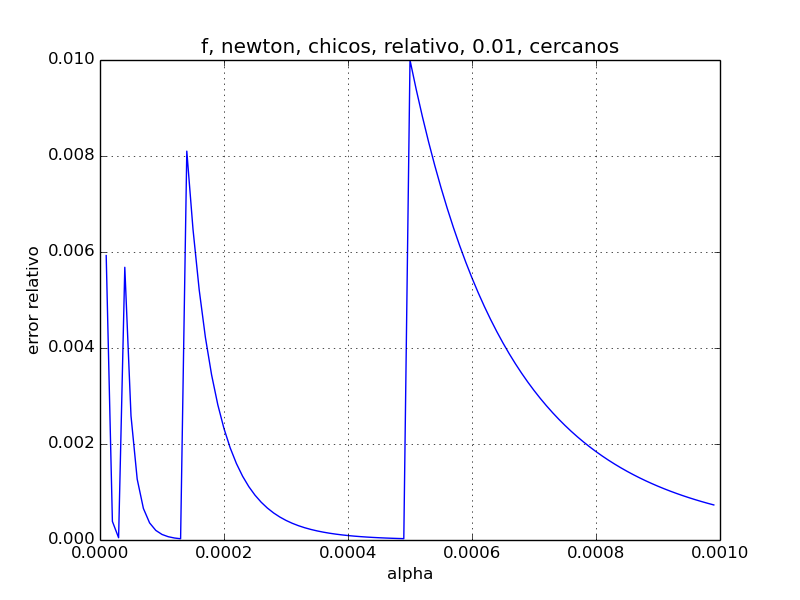
\includegraphics[scale=0.5]{../codigo/resultados/relativo-f-newton-chicos-relativo-0.01-cercanos.png}\\
%$f(x)$ con Newton con $\alpha$'s chicos y $x_0 = 0.01$
%\end{center}

Veamos algunos resultados graficamente:

\subsection{Cantidad de iteraciones f(x) con Newton y Secante}
Estos gráficos fueron generados con un inputs similares. En el caso de secante se utilizó el mismo $x_0$ y para $x_1 = 2x_0$. Podemos ver que ambos gráficos se comportan similarmente, a medida que el $x_0$ crece, crece la cantidad de iteraciones.\\

\begin{center}
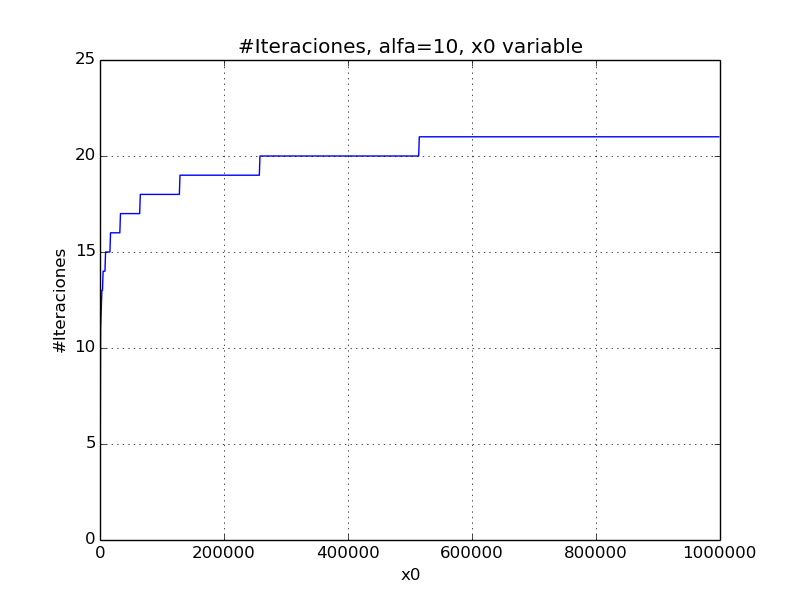
\includegraphics[scale=0.5]{graficos/iteraciones-f-newton-alfa_fijo-absoluto-0.001-alejando.png}\\
$f(x)$ aproximada con Newton, criterio de parada error absoluto igual a $0.001$
\end{center}

\begin{center}
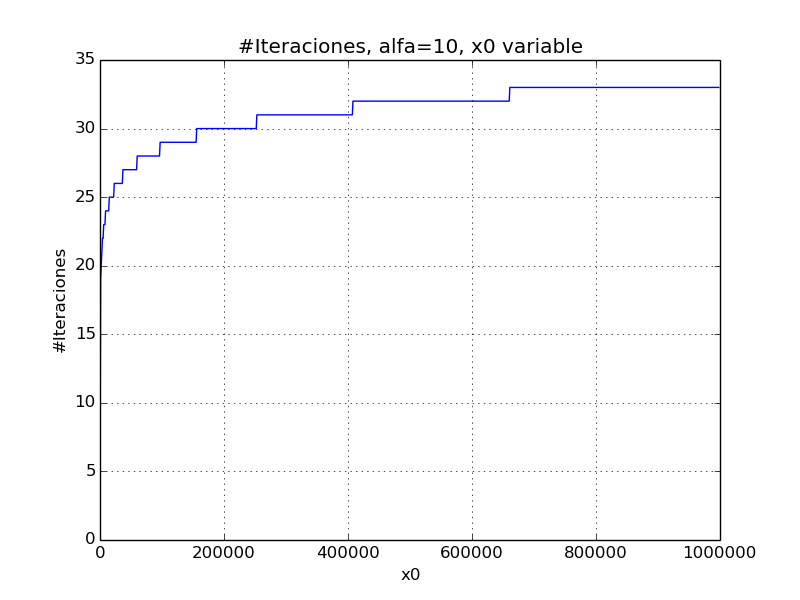
\includegraphics[scale=0.5]{graficos/iteraciones-f-secante-alfa_fijo-absoluto-0.001-alejando.png}\\
$f(x)$ aproximada con Newton, criterio de parada error absoluto igual a $0.001$
\end{center}

\subsection{Error Absoluto f(x) con Newton y Secante}
Al igual que en los gráficos anteriores acá también se realizaron las pruebas con inputs similares.\\

\begin{center}
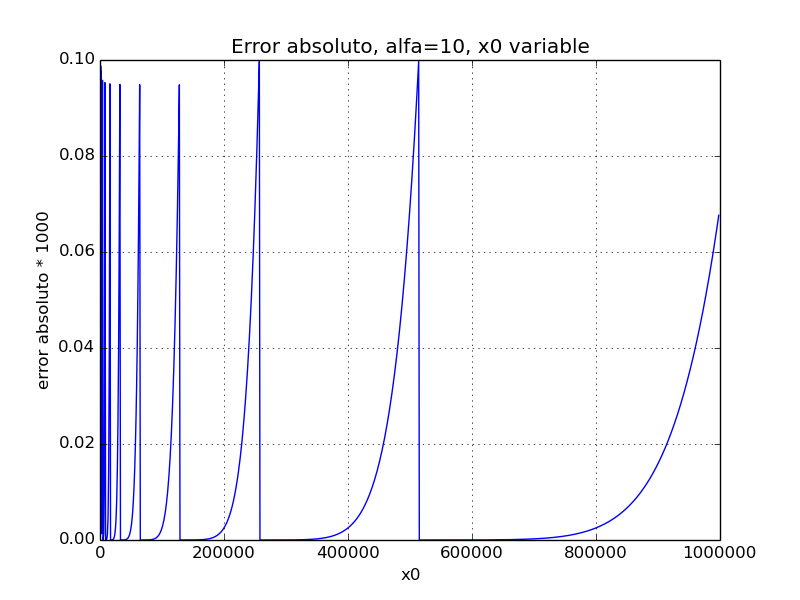
\includegraphics[scale=0.5]{graficos/x0s-f-newton-alfa_fijo-absoluto-0.001-alejando.png}\\
Newton. Criterio de parada: Error absoluto igual a 1 $\times$ $10^{-3}$
\end{center}

\begin{center}
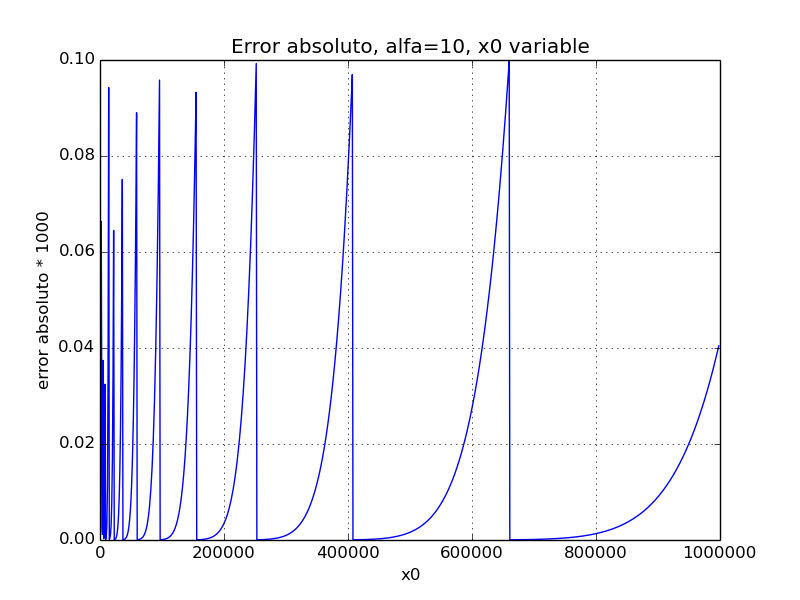
\includegraphics[scale=0.5]{graficos/x0s-f-secante-alfa_fijo-absoluto-0.001-alejando.png}\\
Secante. Criterio de parada: Error absoluto igual a 1 $\times$ $10^{-3}$
\end{center}


\subsection{Tiempo de Computo f(x) con Newton y Secante}
Nuevamente se utilizaron inputs similares para ambos gráficos. La idea era comparar los tiempos de CPU para cada método.
\begin{center}
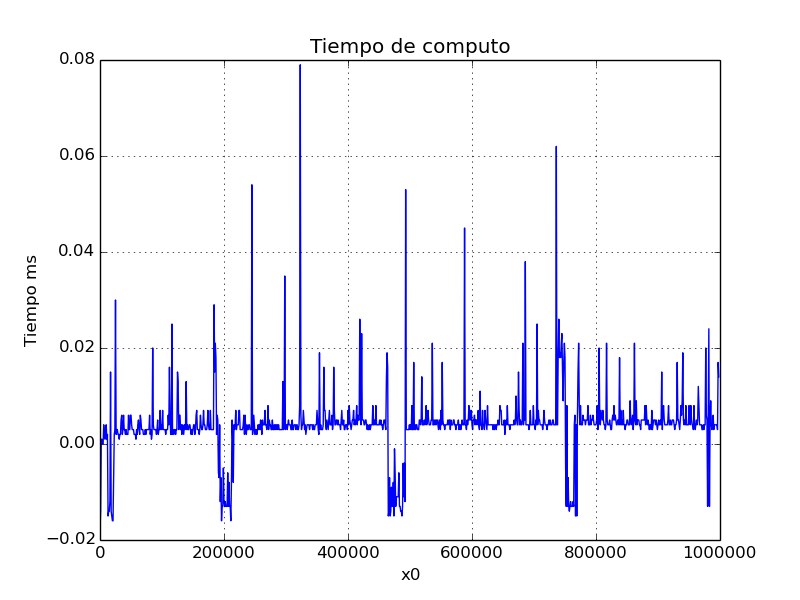
\includegraphics[scale=0.5]{graficos/tiempo-f-newton-alfa_fijo-absoluto-0.001-alejando.png}\\
Newton con $\alpha$ fijo y error absoluto de $0.001$ con $x_0$ creciente.
\end{center}

\begin{center}
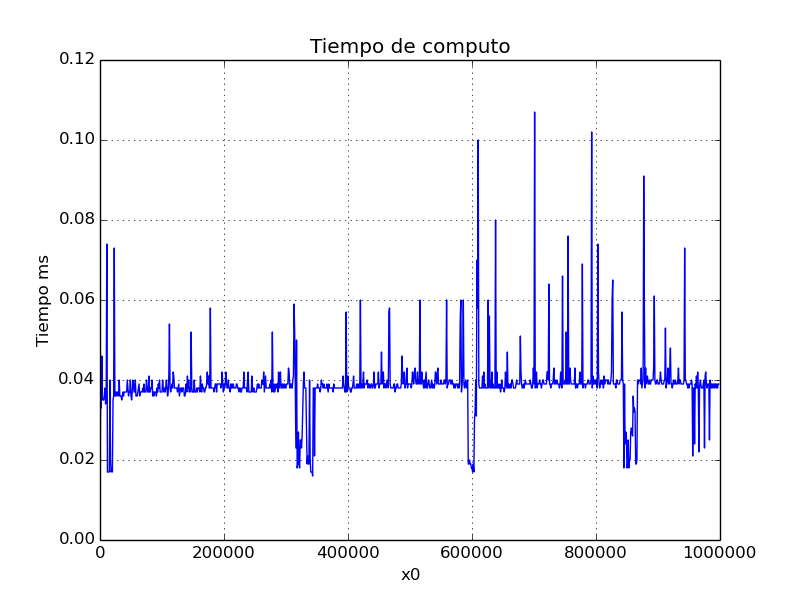
\includegraphics[scale=0.5]{graficos/tiempo-f-secante-alfa_fijo-absoluto-0.001-alejando.png}\\
Secante con $\alpha$ fijo y error absoluto de $0.001$ con $x_0$ creciente.
\end{center}

\subsection{Graficos para f(x) con error absoluto 0.0001}

\begin{center}
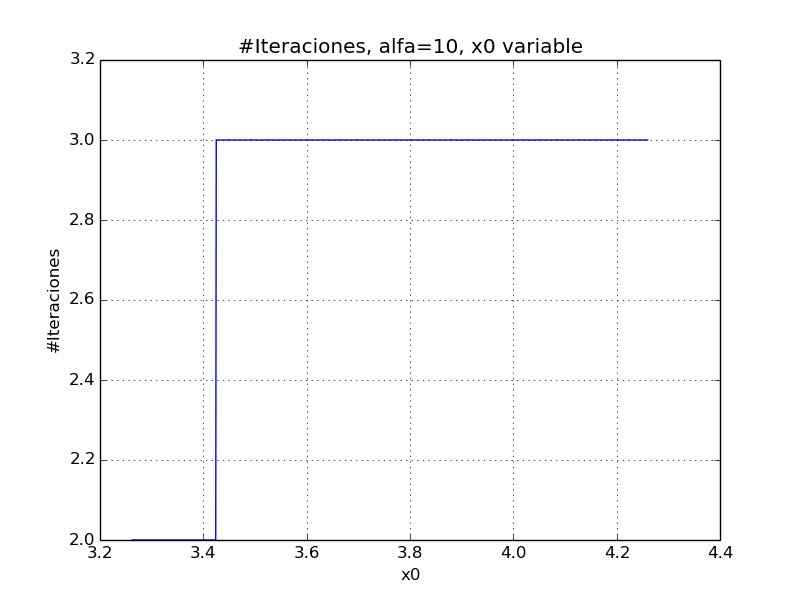
\includegraphics[scale=0.5]{graficos/iteraciones-f-newton-alfa_fijo-absoluto-0.0001-alejando_cercano.png}\\
poner titulo
\end{center}

\begin{center}
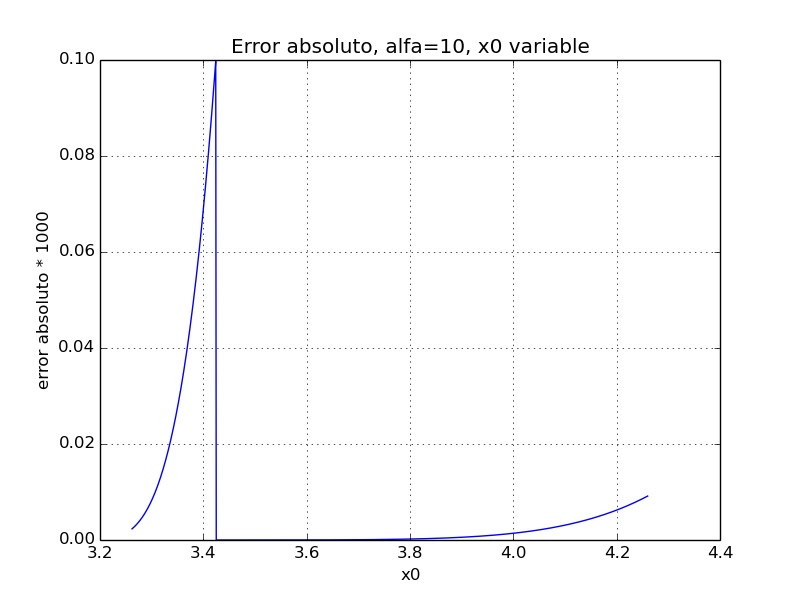
\includegraphics[scale=0.5]{graficos/x0s-f-newton-alfa_fijo-absoluto-0.0001-alejando_cercano.png}\\
poner titulo
\end{center}

\begin{center}
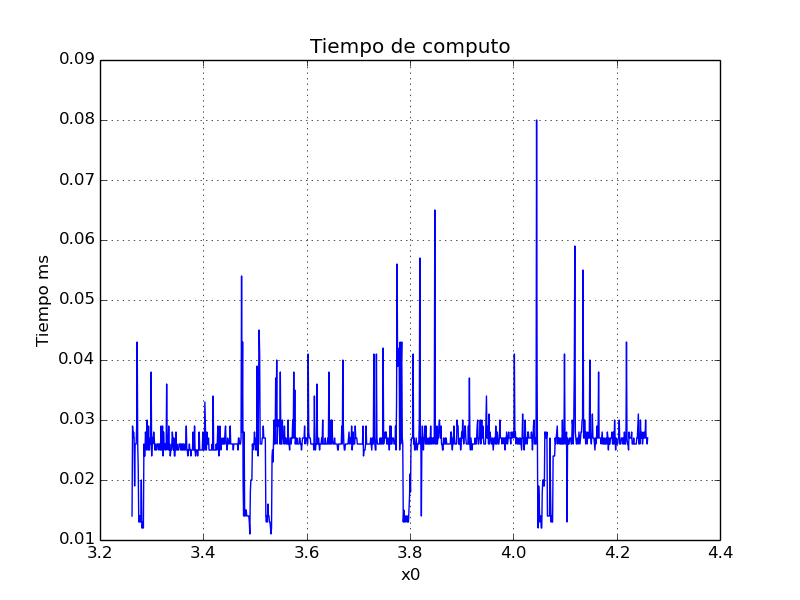
\includegraphics[scale=0.5]{graficos/tiempo-f-newton-alfa_fijo-absoluto-0.0001-alejando_cercano.png}\\
poner titulo
\end{center}

\subsection{Graficos para e(x)}

Los $x_0$ y $x_1$ se tomaron en $\frac{1}{\sqrt{\alpha}} + 0.001$ y superiores y $-\frac{1}{\sqrt{\alpha}} - 0.001$

Se observa que la función converge solo para un intervalo limitado, probablemente debido a que la función tiene dos asíntotas, y su derivada en los límites al infinito tiende a cero, dificultando cálculos por números demasiado grandes y demasiado chicos.

Se ve que el comportamiento es errático y difícil de predecir, en comparación a la resolución del inverso.

Las mismas observaciones sobre la dificultad de medir el tiempo de ejecución se aplican aquí.


------------------------
\begin{center}
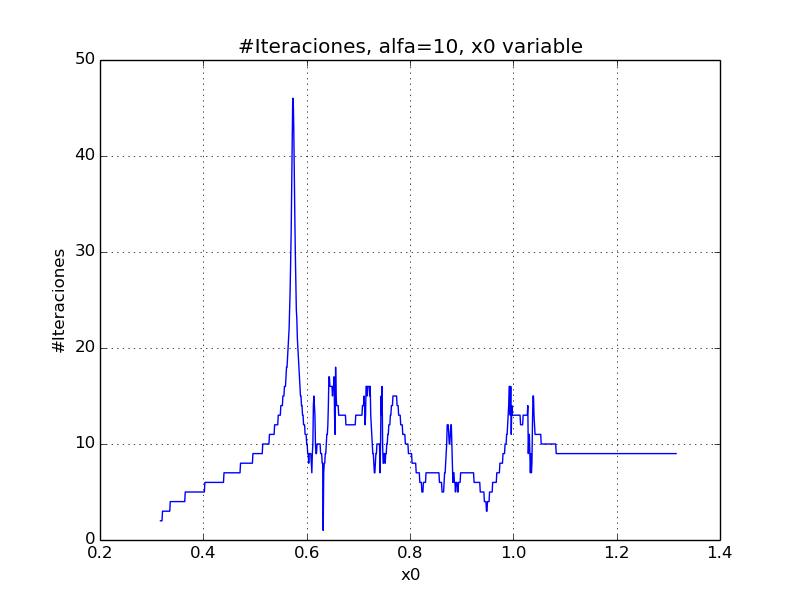
\includegraphics[scale=0.5]{graficos/iteraciones-e-secante-alfa_fijo-absoluto-0.0001-alejando.png}\\
poner titulos
\end{center}
------------------------
\begin{center}
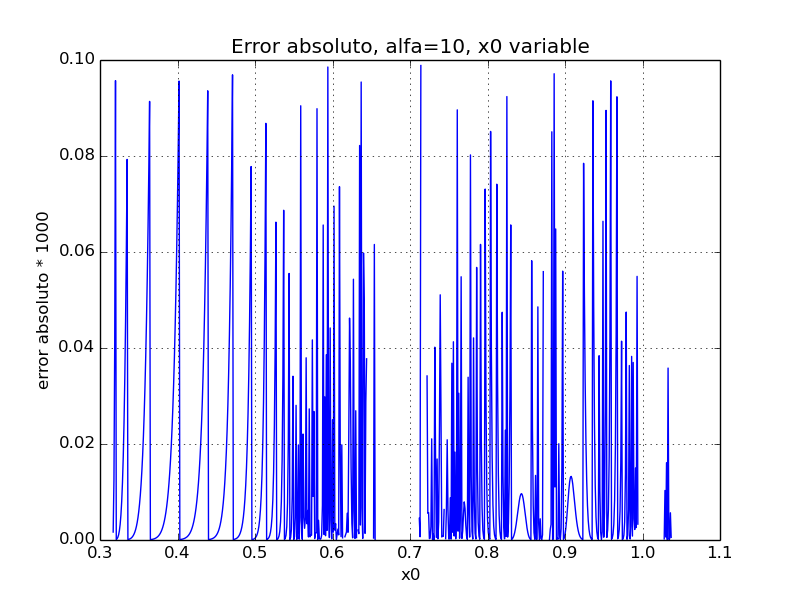
\includegraphics[scale=0.5]{graficos/x0s-e-secante-alfa_fijo-absoluto-0.0001-alejando.png}\\
poner titulos
\end{center}
------------------------
\begin{center}
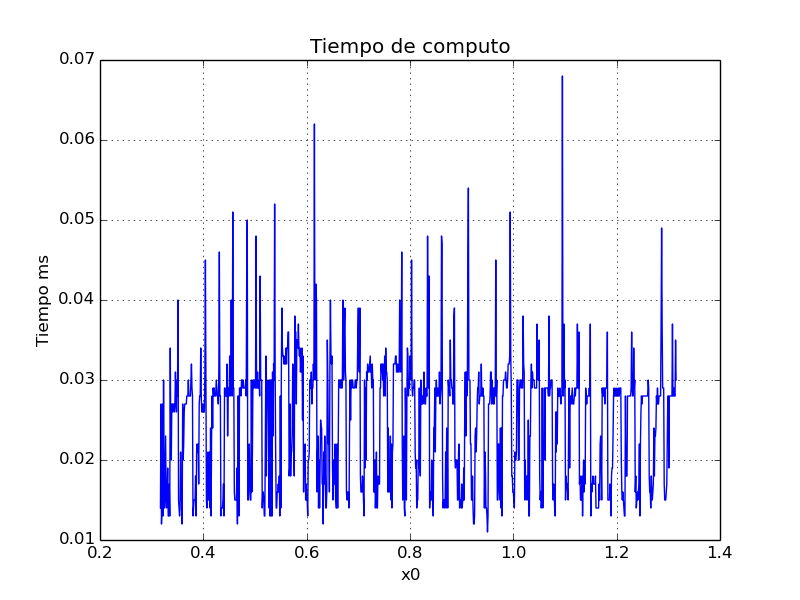
\includegraphics[scale=0.5]{graficos/tiempo-e-secante-alfa_fijo-absoluto-0.0001-alejando.png}\\
poner titulos
\end{center}
------------------------
\begin{center}
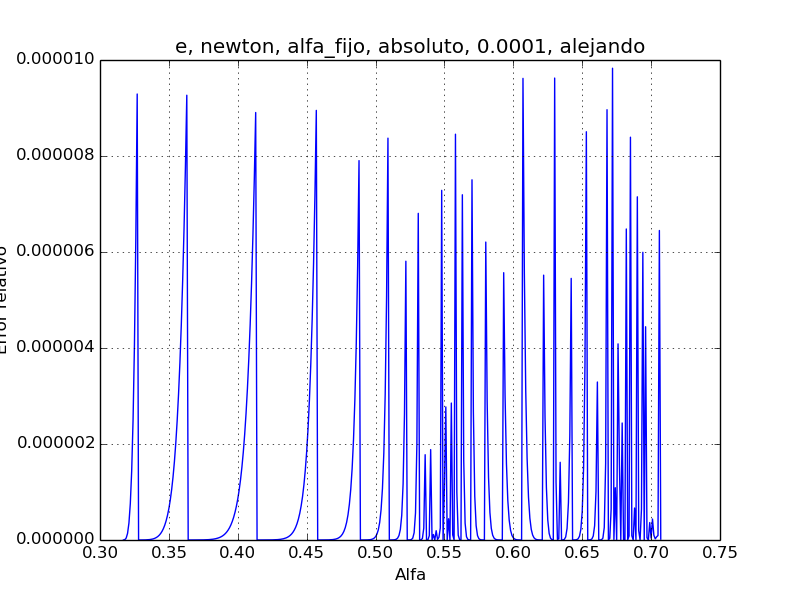
\includegraphics[scale=0.5]{graficos/relativo-e-newton-alfa_fijo-absoluto-0.0001-alejando.png}\\
poner titulos
\end{center}
------------------------
\begin{center}
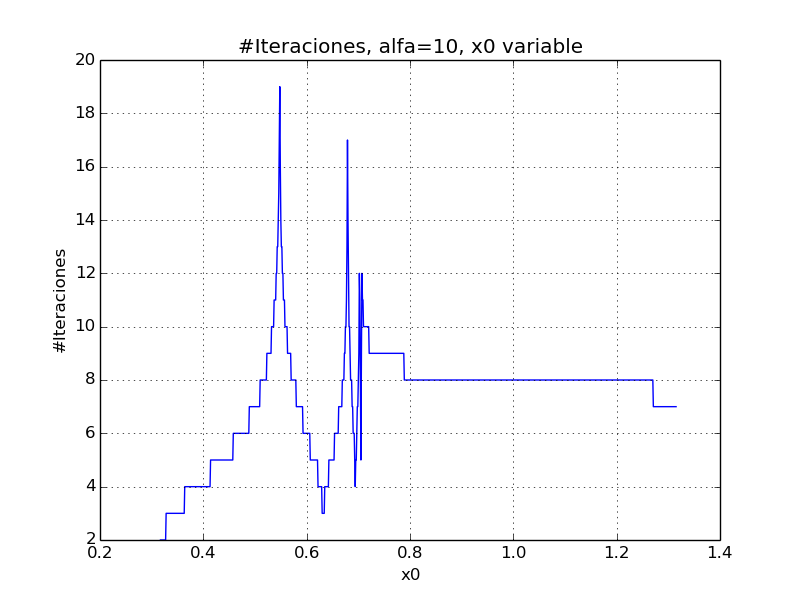
\includegraphics[scale=0.5]{graficos/iteraciones-e-newton-alfa_fijo-absoluto-0.0001-alejando.png}\\
poner titulos
\end{center}
------------------------
\begin{center}
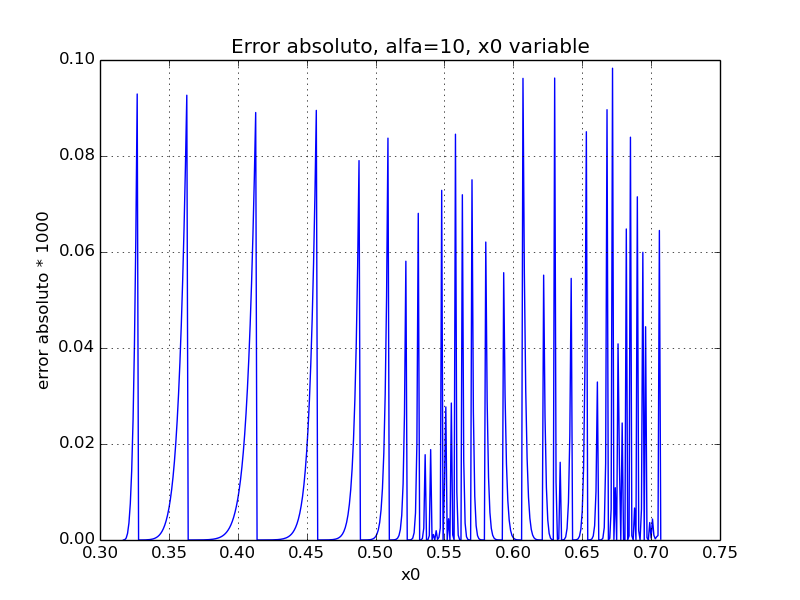
\includegraphics[scale=0.5]{graficos/x0s-e-newton-alfa_fijo-absoluto-0.0001-alejando.png}\\
poner titulos
\end{center}
------------------------
\begin{center}
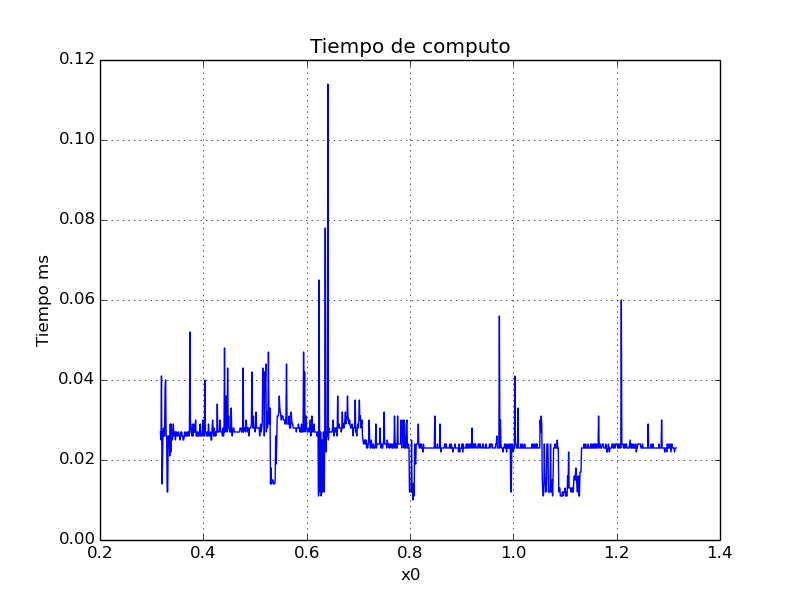
\includegraphics[scale=0.5]{graficos/tiempo-e-newton-alfa_fijo-absoluto-0.0001-alejando.png}\\
poner titulos
\end{center}
------------------------







% Ver un grafico que muestra los picos del error relativo conforme el alapha se aleja del x0. La explicacion es que conforme mas lejos esta el x0 del resultado, tiene que realizar mas itreraciones y el error relativo de la ultima iteracion que vale crece conforme aumenta la distancia entre alpah y x0 hasta que la iteracion no califica para entrar en el criterio de tension relativo. Entonces debe realizar una iteracion mas que resulta mas precisa y asi sucesivamente

% Hay que un hacer un grafico del mismo experimento pero con el numero de iteraciones y queremos mosrtar que conforme la distancaio del x0 al alpha crece pasa que la cant de iteraciones para converger aumenta.

% Hacer un exp de un alpha fijo con un x0 que se va corriendo. Para observar las iteraciones sobre un valor fijo con la distancia entre x0 y alpha, corriendo el x0. Ademas un grafico de tiempo.

% Un grafico de newton de 1 al 10000 con error absoluto con x0 cercanos al resultado real y compararlo con las iteraciones del relativo

%Los tipos de experimentos:
%* Comparar newton y secante para f(x) y e(x) en función de:
%    1. cantidad de iteraciones
%    2. tiempo de ejecución
%    3. error relativo, error absoluto
%    4. orden de convergencia
%* Los tipos de inputs a utilizar pueden ser:
%    1. crecientes de 1 a 1000 en intervalos de 1, 5 y 10
%    2. crecientes de 0 a 1 en intervalos chiquitos, la idea es ver cuando forzamos a que la precisión se pierda
%    2. aleatorios con magnitud definida